\chapter{Biologia Molecular e Bioinformática}
\label{sec:BiologiaMolecularBioInformática}

Neste capítulo, serão apresentados conceitos básicos de Biologia Molecular e Bioinformática, necessários ao entendimento deste trabalho. Na Seção \ref{sec:AcidosNucleicos}, são apresentados os ácidos nucléicos, que contêm informações e mecanismos para sintetizar proteínas. Na Seção \ref{sec:Dogma}, descrevemos o Dogma Central da Biologia Molecular, ou o processo através do qual as informações contidas no DNA, através de diversos tipos de RNAs, são utilizados para a síntese de proteínas. Na Seção \ref{sec:pipeline} particularmente descreve mas técnicas de sequenciamento de genomas e os \textit{pipelines} associados.


\subsection{Ácidos nucléicos} \label{sec:AcidosNucleicos}

Os ácidos nucléicos são polímeros formados a partir de moléculas mais simples, chamadas de nucleotídeos. Um nucleotídeo tem na sua composição açúcar com cinco átomos de carbono (pentose), ligado a um grupo fosfato e uma base nitrogenada~\citep{koolman:2005}, como podemos ver na Figura~\ref{fig:AcidosNucleicos}.

\begin{figure}[ht]
\centering
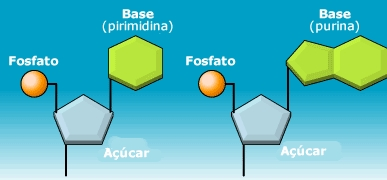
\includegraphics[angle=0,width=0.55\textwidth]{imagens//AcidosNucleicos.jpg}
\caption{Estrutura esquemática de um nucleotídeo, mostrando seus principais componentes: açúcar, fosfato e base nitrogenada~\citep{brainstuff:2000}. \label{fig:AcidosNucleicos}}
\end{figure}

A síntese dos ácidos nucléicos envolve ligações entre diferentes nucleotídeos, atráves dos grupos fosfato, por meio de uma ligação chamada ligação fosfodiéster. Nessa ligação, o átomo de fósforo estabelece fortes ligações covalentes com os átomos de carbono da pentose dos nucleotídeos.


\subsubsection{DNA} \label{sec:DNA}

O ácido desoxirribonucléico (DNA) contém as informações genéticas de um organismo vivo, com exceção de alguns vírus~\citep{silva:2001}. Nos organismos procariotos, o material genético está espalhado na célula. Nas células eucarióticas, o DNA está localizado no núcleo, e contém informações sobre como, quando e onde produzir cada tipo de proteína~\citep{lodish:2005}.


Uma molécula de DNA é formada por cadeias de nucleotídeos. As bases nitrogenadas, as quais constituem os nucleotídeos, podem ser divididas em dois grupos: purinas ou pirimidinas. Nas bases purinas encontram-se as bases formadas por dois anéis, a citosina (C) e a timina (T) e nas pirimidinas encontram-se as bases formas por anéis, a Adenina (A) e a Guanina (G).
Assim, existem quatro tipos de nucleotídeos, de acordo com sua base nitrogenada Figura~\ref{fig:nucleotideoDNA}, onde P representa o grupo fosfato, D a pentose (açúcar denominado de desoxirribose) as bases nitrogenadas que podem ser A, G, C ou T.

\begin{figure}[ht]
\centering
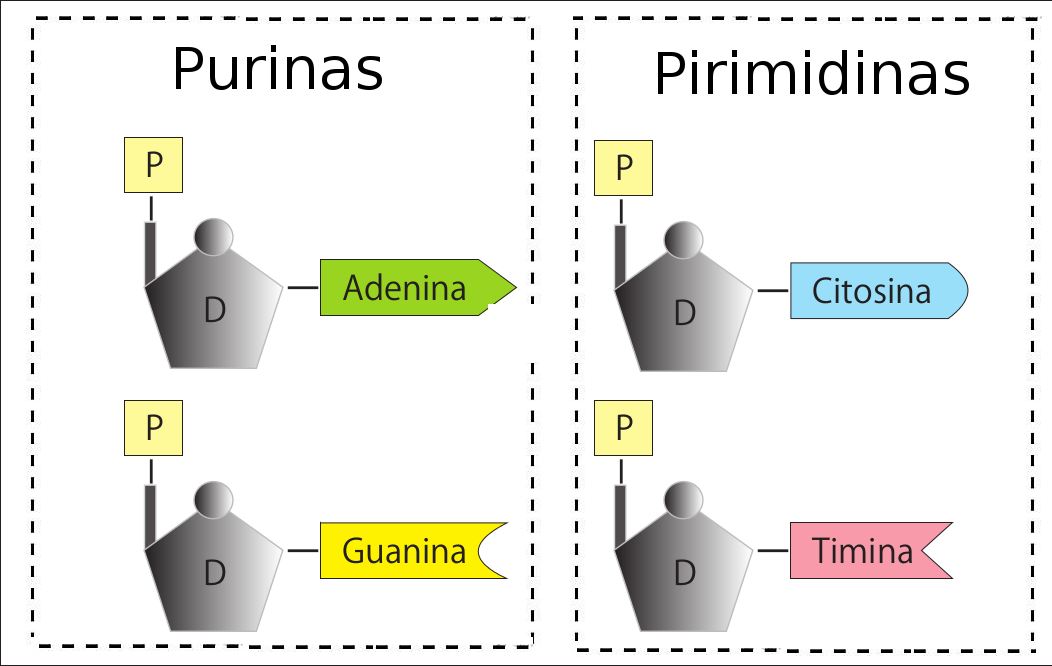
\includegraphics[angle=0,width=0.5\textwidth]{imagens//2007eu-nucleotideoDNA1}
\caption{Os quatros tipos de nucleotídeos que compõem a molécula de DNA.\label{fig:nucleotideoDNA}}
\end{figure}

A estrutura do DNA é formada por duas cadeias ou fitas paralelas compostas por uma sequência de nucleotídeos, que são unidas através de pontes de hidrogênio formadas entre as bases nitrogenadas de cada fita, onde a base A estará pareada com a base T (A-T) e C com G (C-G)~\citep{stryer:2002}. As bases A-T e C-G são chamadas de bases complementares. Essas duas fitas estão dispostas em espiral em torno de um eixo. Cada fita possui uma extremidade chamada 5' e a outra chamada 3', o que cria uma orientação em cada uma das fitas. As duas cadeias ficam, portanto em direção antiparalelas (opostas), formando uma dupla-hélice Figura~\ref{DNA-replicacao}.


O DNA pode sofrer replicações em alguns momentos através de um processo conhecido como duplicação semiconservativa, onde cada DNA recém formado possui uma das cadeias da molécula mãe~\citep{lopes:1998}.
Para realizar a replicação, a dupla fita do DNA abre-se, através do rompimento das pontes de hidrogênio, e os nucleotídeos livres encaixam-se na molécula através de novas pontes de hidrogênio. Os nucleotídeos vão sendo ligados entre si pela enzima DNA polimerase. O resultado desse processo é a formação de duas moléculas de DNA idênticas à original Figura~\ref{DNA-replicacao}.

\begin{figure}[ht]
\centering
\fbox{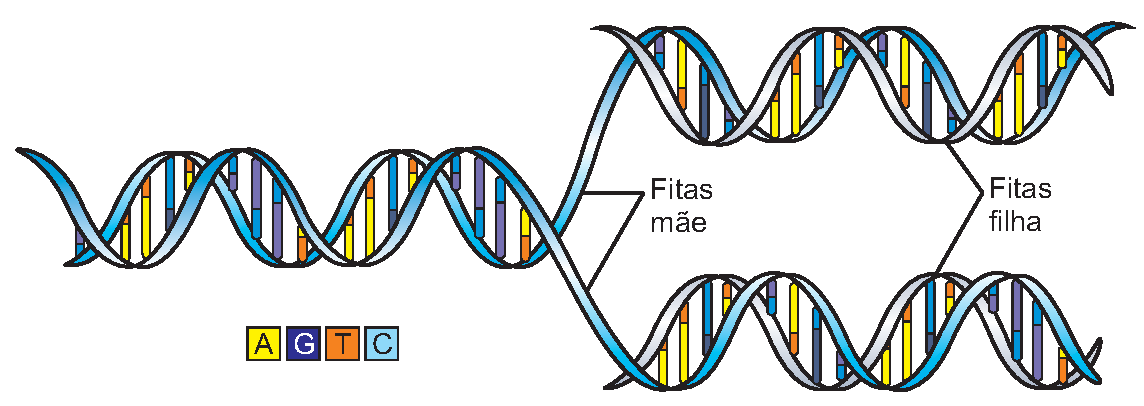
\includegraphics[angle=0,width=0.7\textwidth]{imagens//2005lodish-DNA-replicacao.pdf}}
\caption{Replicação DNA Semiconservativa. À esquerda podemos observar um trecho de uma molécula de DNA que evidencia o aspecto de dupla-hélice e à direita as fitas mãe separadas, servindo de molde para as filhas, resultando em duas moléculas idênticas à dupla-hélice original~\citep{lodish:2005}. \label{DNA-replicacao}}
\end{figure}

%\newpage
Algumas regiões do DNA possuem informações para codificar proteínas ou ncRNAs e são chamadas de genes. Esses genes são transcritos em RNAs, que realizam diversas funções, como catalíticas ou estruturais para síntese de proteínas ou regulação. Assim, a sequência de nucleotídeos do DNA é chamada de estrutura primária, ou seja, a estrutura primária é dada pela sequência linear formada ao longo da cadeia, sendo o nível estrutural mais simples~\citep{lodish:2005}. A estrutura secundária consiste no arranjo espacial da sequência.


\subsubsection{RNA} \label{sec:RNA}

De forma semelhante ao DNA, o ácido ribonucléico (RNA) é uma molécula constituída por cadeias de nucleotídeos, ou polinucleotídeo.


O RNA é também formado pelo grupo fosfato, açúcar (ribose) e por uma base nitrogenada. Porém, entre as bases nitrogenadas, a Uracila (U) substitui a Timina (T) do DNA~\citep{lodish:2005}. Assim, U é uma base purina. Na Figura~\ref{fig:nucleotideoRNA}, P representa o grupo fosfato, R a ribose e, em seguida, as bases nitrogenadas A, G, C e U.

\begin{figure}[ht]
\centering
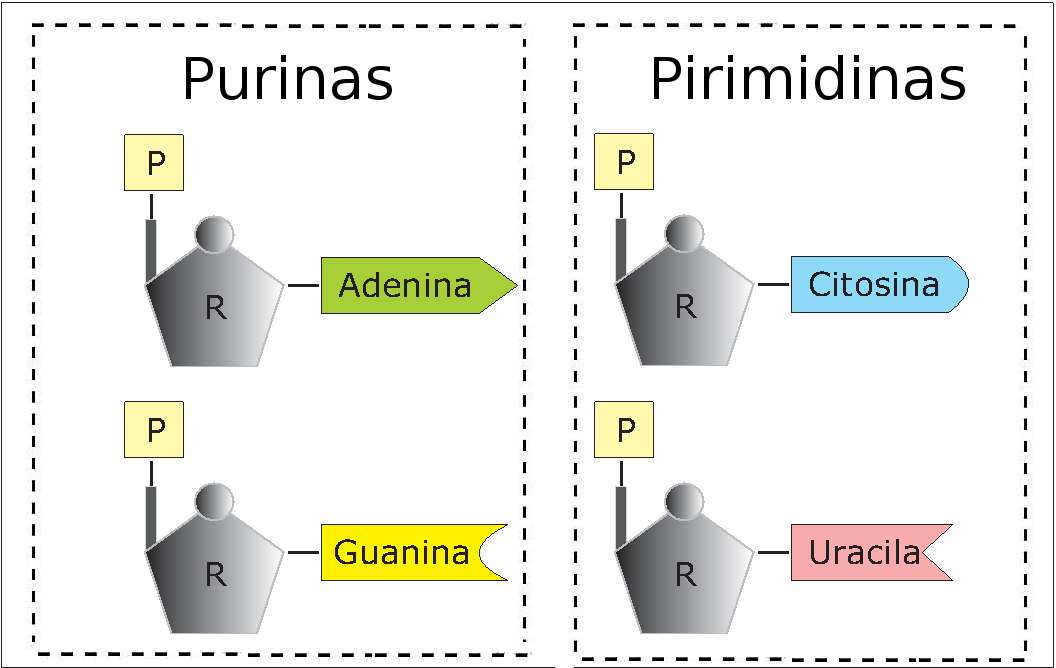
\includegraphics[angle=0,width=0.5\textwidth]{imagens//2007eu-nucleotideoRNA1}
\caption{Tipos de nucleotídeos que compõem a molécula de RNA, observando-se que a Uracila (U) substitui a Timina (T) nos RNAs. \label{fig:nucleotideoRNA}}
\end{figure}


O RNA é formado em geral por uma única fita de nucleotídeos, e não possui o aspecto de dupla-hélice~\citep{koolman:2005}. Porém, como o RNA tem como bases complementareas (A-U) e (C-G), pode unir-se através de pontes de hidrogênio, ou seja, o RNA pode dobrar-se.

Na síntese de proteínas estão envolvidos três tipos de RNAs, descritos com mais detalhes na Seção~\ref{sec:Dogma}: o mensageiro (mRNA), o ribossômico (rRNA) e o transportador (tRNA).


A Figura~\ref{fig:rRNA} mostra uma estrutura de um rRNA 16S da bactéria \textsl{Escherichia coli}. Esse RNA é o componente central dos ribossomos, que são organelas encontradas no citoplasma possuindo duas subunidades chamadas de 40S e 60S em células eucarióticas e 30S e 50S em bactérias~\citep{lafontaine:2001}. O mRNA é encontrado tanto no núcleo (onde ocorre sua síntese) quanto no citoplasma (onde participa da tradução de proteínas). Por último, vamos falar sobre os tRNAs, que são encontrados no citoplasma e funcionam durante a tradução, fazendo as ligações entre as proteínas e ácidos nucléicos. Esses RNAs são pequenos, contendo entre 70 e 90 nucleotídeos~\citep{koolman:2005}.

\begin{figure}[htb!]
\centering
\fbox{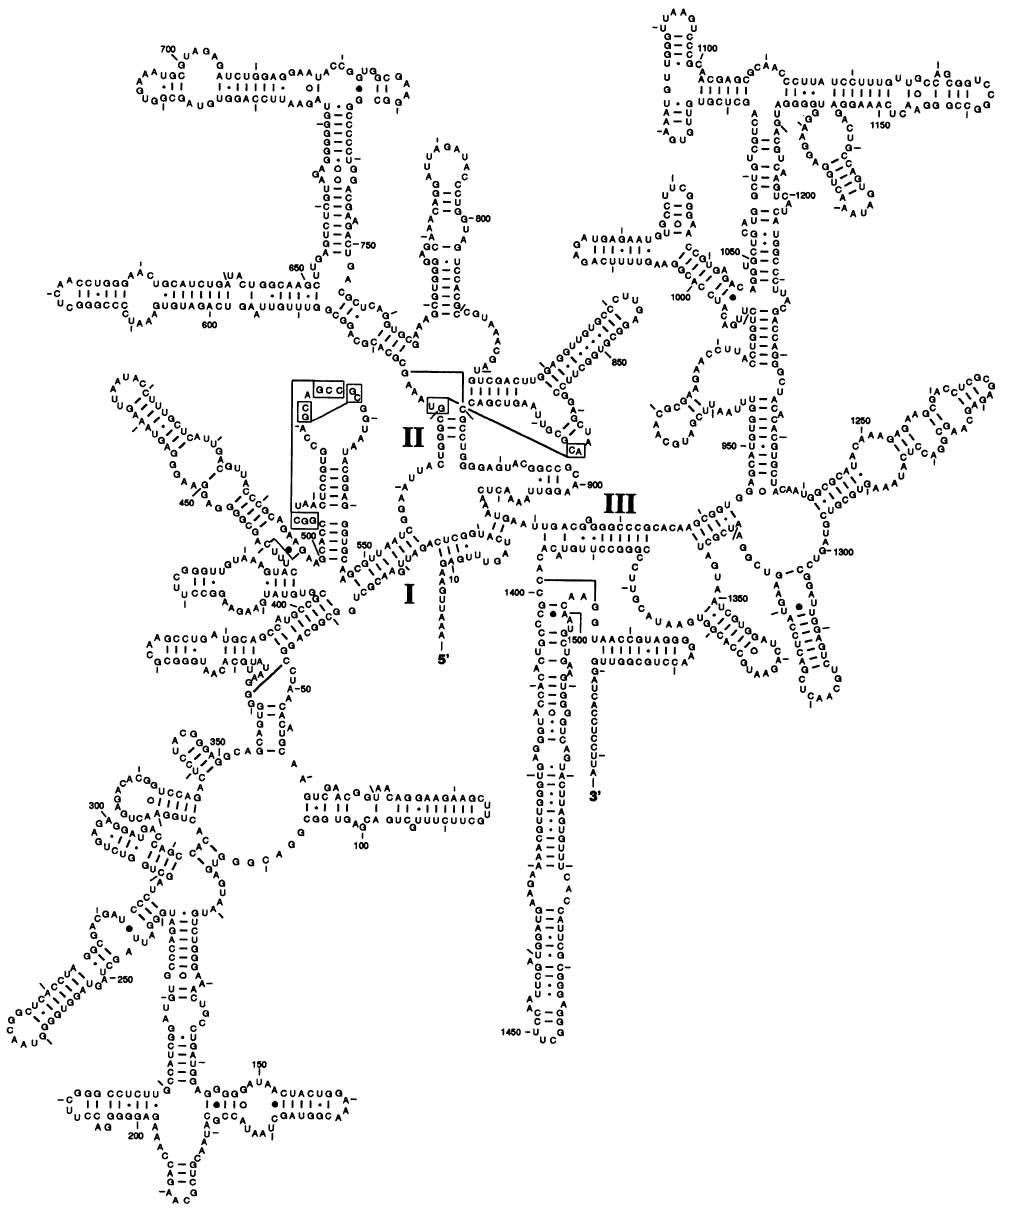
\includegraphics[angle=0,width=1.0\textwidth]{imagens//1994gutell-rRNA.jpg}}
\caption{Modelo da estrutura de um rRNA 16S da E.coli~\citep{gutell:1994}. \label{fig:rRNA}}
\end{figure}


\newpage
\subsection{Dogma Central da Biologia Molecular: Síntese de Proteínas}  \label{sec:Dogma}  % 2.4

Nesta seção, mostraremos como as informações presentes em uma molécula de DNA são utilizadas na síntese de proteína.


Em primeiro lugar, a transcrição ocorre no núcleo, e é sintetizada pela enzima RNA polimerase, que vai ligar-se a uma determinada sequência de nucleotídeos do DNA, identificadas pelas regiões promotoras, e a percorre utilizando-a como molde até encontrar as regiões terminadoras. A transcrição baseia-se no pareamento de bases complementares usando uma fita do DNA como molde, ou seja, adenina com uracila (A $\rightarrow$ U), timina com adenina (T $\rightarrow$  A) e citosina com guanina (C $\leftrightarrow$ G). A molécula de RNA recém sintetizada é o mRNA~\citep{lodish:2005}.

O processo de transcrição acontece tanto nos procariotos (não possuem núcleo celular) Figura~\ref{fig:processo-sintese-proteinaProc} como nos eucariotos (tem o DNA armazenado em um núcleo celular), tendo seu processo de transcrição um pouco mais complexo que os procariotos.

De acordo com~\citep{lodish:2005}, todos os organismos possuem maneiras de controlar quando os seus genes podem ser transcritos. Muitas células são capazes de responder a sinais externos ou a alterações nas condições externas, ligando ou desligando genes específicos, dessa forma, as células adaptam-se às necessidades do momento.

\begin{figure} [htb!]
\centering
\fbox{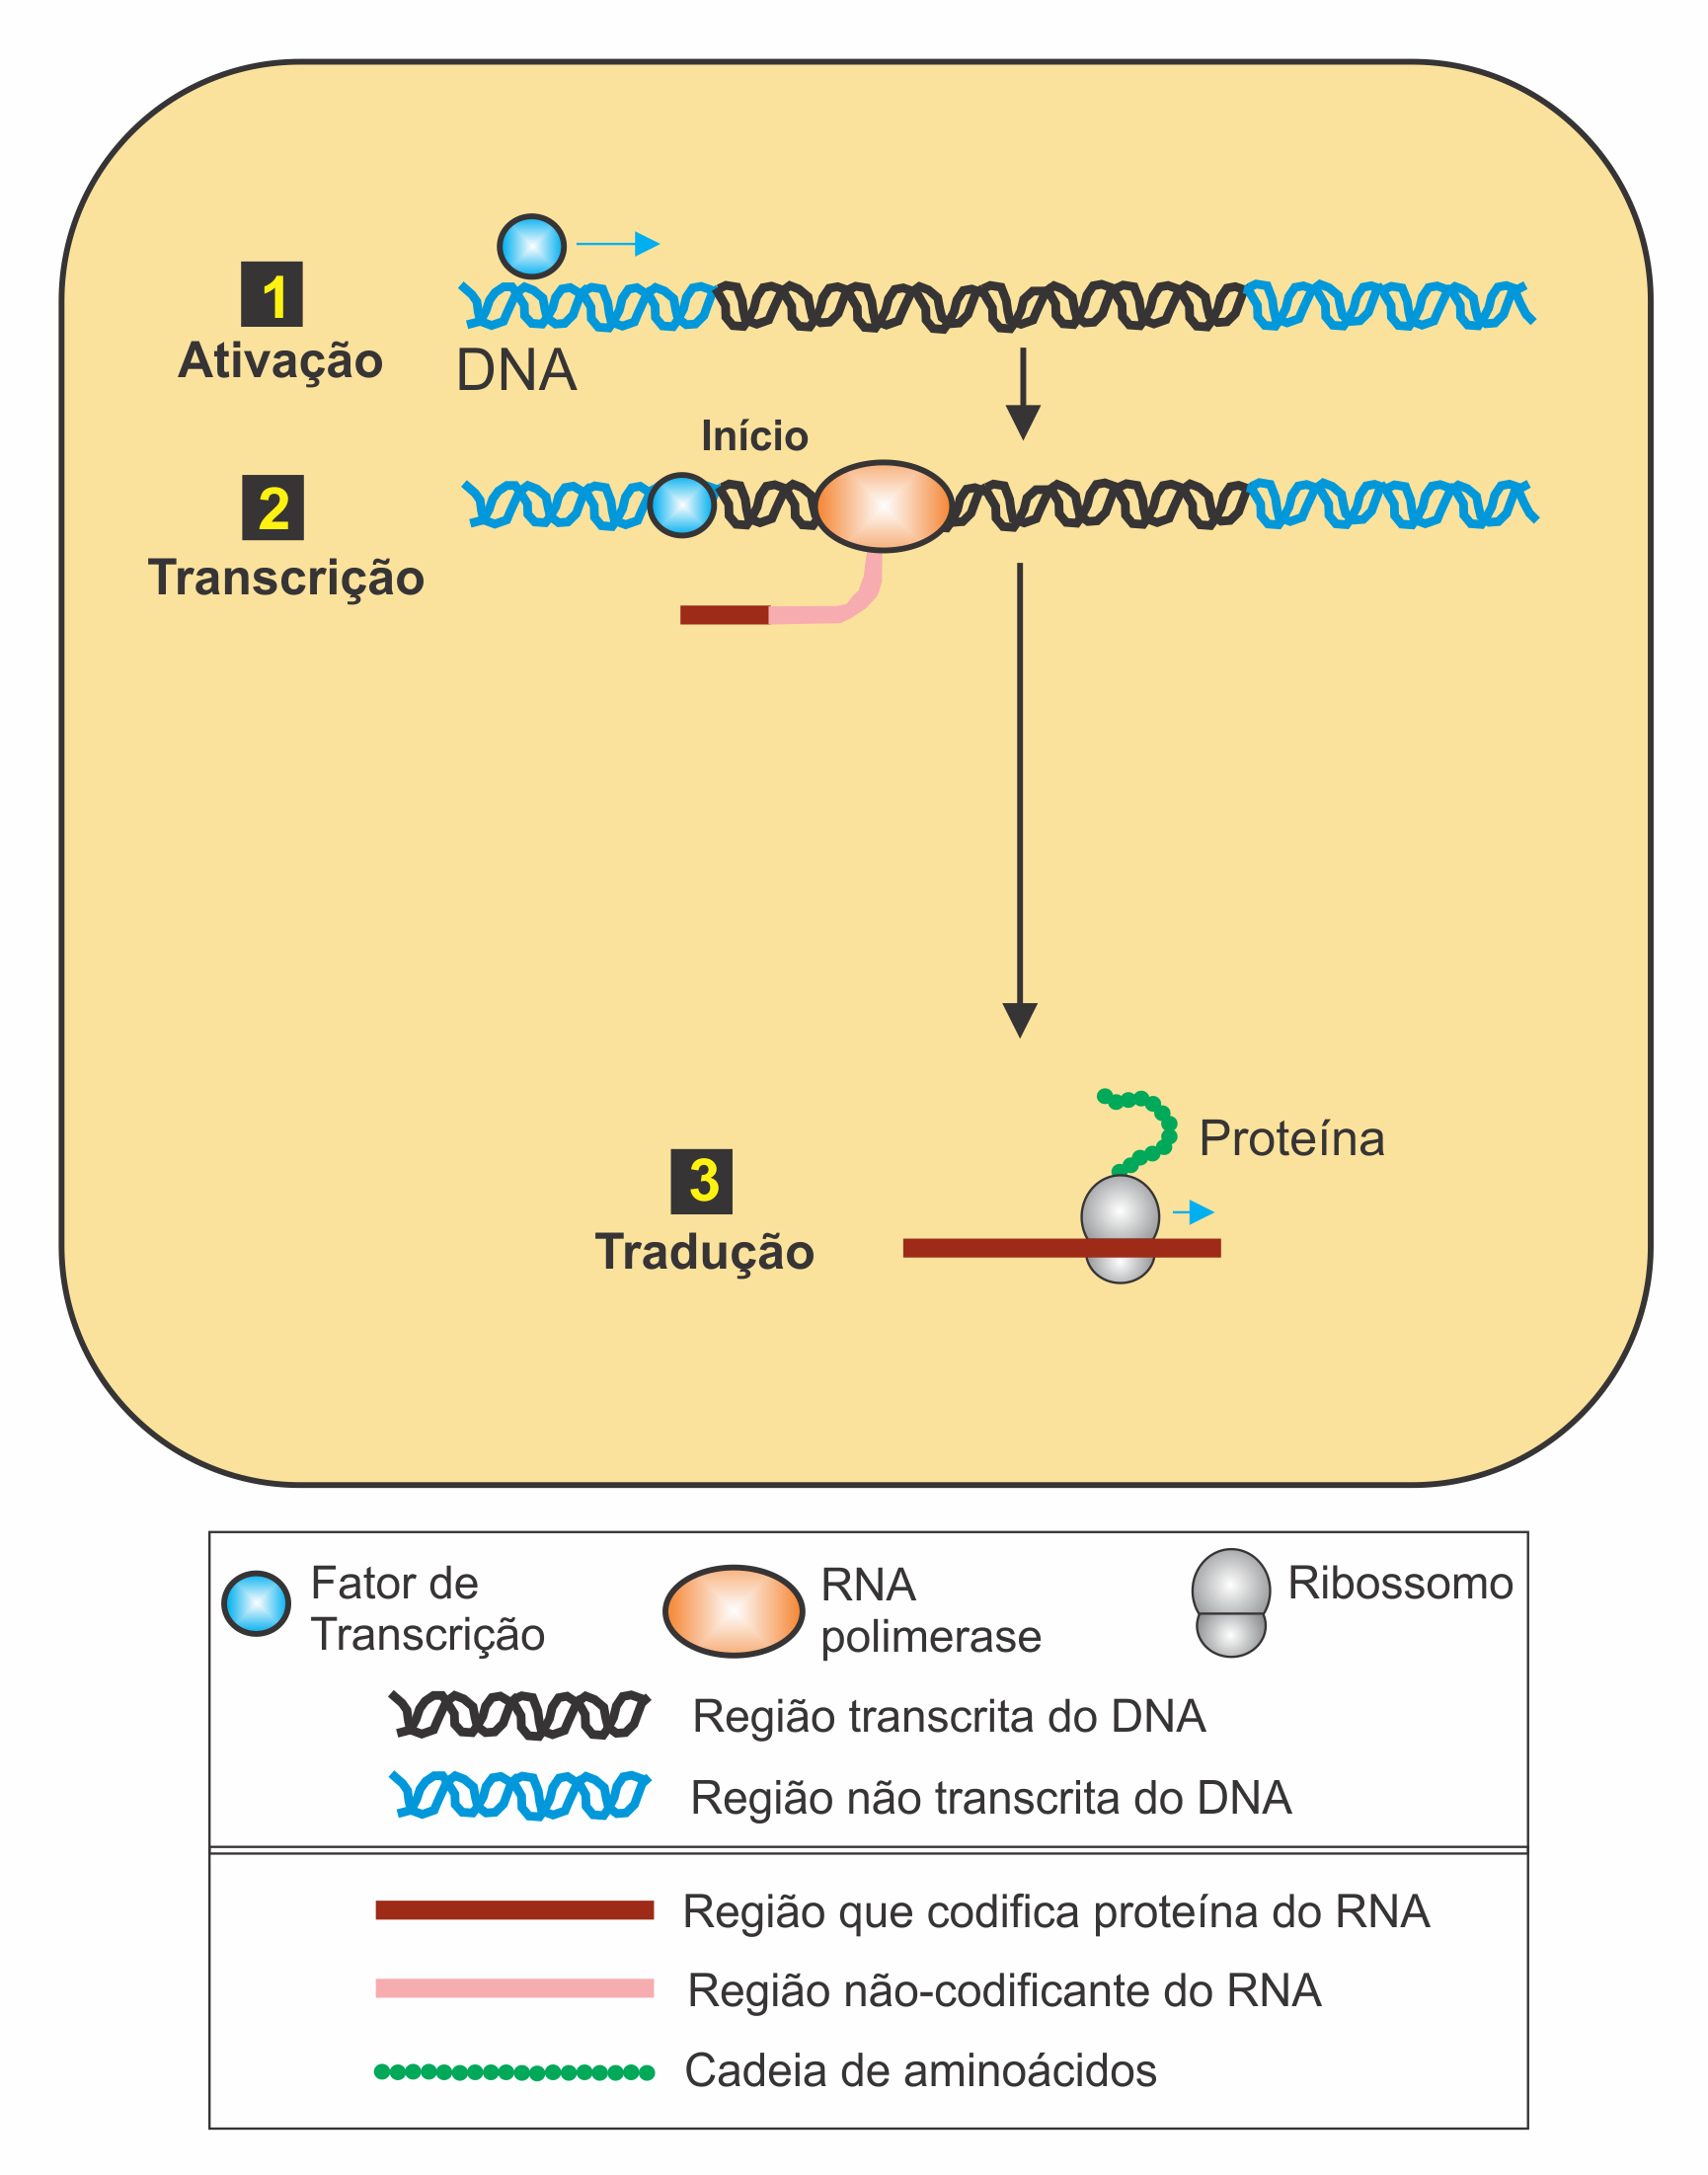
\includegraphics[angle=0,width=0.8\textwidth]{imagens//2005lodish-DNA-transcricao-traducaoProca.png}}
\caption{A síntese protéica em célula procariótica funciona da seguinte maneira. No passo 1, fatores de transcrição ligam-se às regiões da regulação dos genes que controlam, ativando-os. No passo 2, a RNA polimerase começa a transcrição do gene ativado pela região promotora, resultando na formação do mRNA. No passo 3, o mRNA e ligado no ribossomos. Nesse ponto, a proteína é sintetizada pelo ribossomo que liga os aminoácidos em uma cadeia linear ~\citep{lodish:2005}. \label{fig:processo-sintese-proteinaProc}}
\end{figure}

Nos eucariotos, o mRNA recém-trancrito é conhecido como pré-mRNA, e em alguns organismos ele irá sofrer algumas modificações antes que se transforme em um mRNA maduro~\citep{silva:2001}. No decorrer desse processo de maturação ocorre o \textsl{splicing} (eliminação dos íntrons do pré-mRNA) Figura~\ref{fig:processo-sintese-proteina}, que são regiões que não codificam a proteína~\citep{lodish:2005, Lundblad:2007}. 

\begin{figure} [htb!]
\centering
\fbox{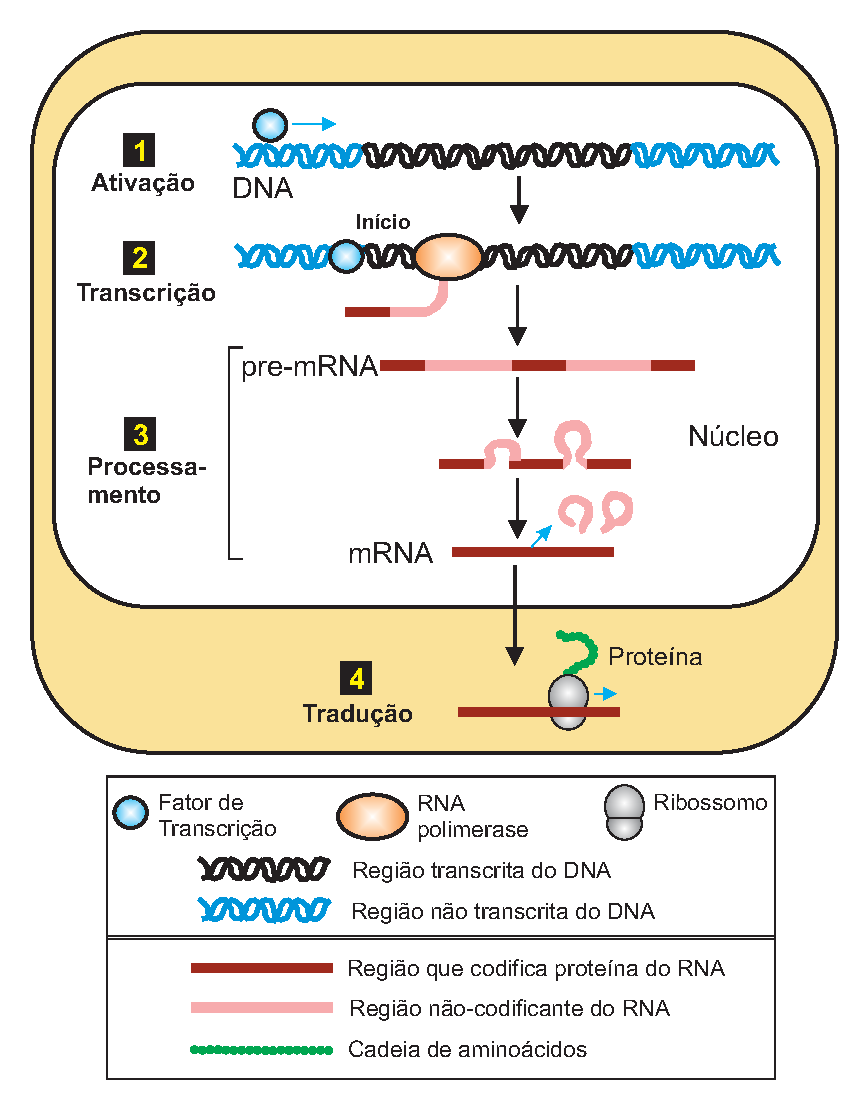
\includegraphics[angle=0,width=0.8\textwidth]{imagens//2005lodish-DNA-transcricao-traducao.pdf}}
\caption{A síntese protéica em célula eucariótica funciona da seguinte maneira. No passo 1, fatores de transcrição ligam-se às regiões da regulação dos genes que controlam, ativando-os. No passo 2, a RNA polimerase começa a transcrição do gene ativado pela região promotora, resultando na formação do pré-mRNA. No passo 3, é feito um processamento na transcrição para remover sequências não-codificadoras. Para finalizar, no passo 4, o mRNA move-se para o citoplasma e é ligado pelo ribossomos. Nesse ponto, a proteína é sintetizada pelo ribossomo que liga os aminoácidos em uma cadeia linear ~\citep{lodish:2005}. \label{fig:processo-sintese-proteina}}
\end{figure}

O mRNA formado através da transcrição move-se para o citoplasma, precisamente nos ribossomos, onde ocorre o segundo processo para a síntese da proteína: a tradução.

\newpage
No processo de tradução, primeiramente o mRNA liga-se entre as duas subunidades do ribossomo, onde cada códon do mRNA é pareado com o anticódon correspondente que está presente em moléculas de tRNA~\citep{silva:2001}. Cada aminoácido é codificado por um grupo de três bases do DNA, recebendo o nome de \textit{tríplex} ou \textit{códon}. Cada códon corresponde a um único aminoácido, porém um mesmo aminoácido pode ser definido por mais de um códon Tabela~\ref{fig:1995voet-aa}~\citep{silva:2001,lopes:1998}. Existem ainda três códons (UAG, UAA e UGA) que não correspondem a nenhum aminoácido, mas idicam sinais de término da tradução~\citep{silva:2001}. 

\begin{table}[ht]
\caption{O Código Genético~\citep{voet:1995}. \label{fig:1995voet-aa}}
\centering
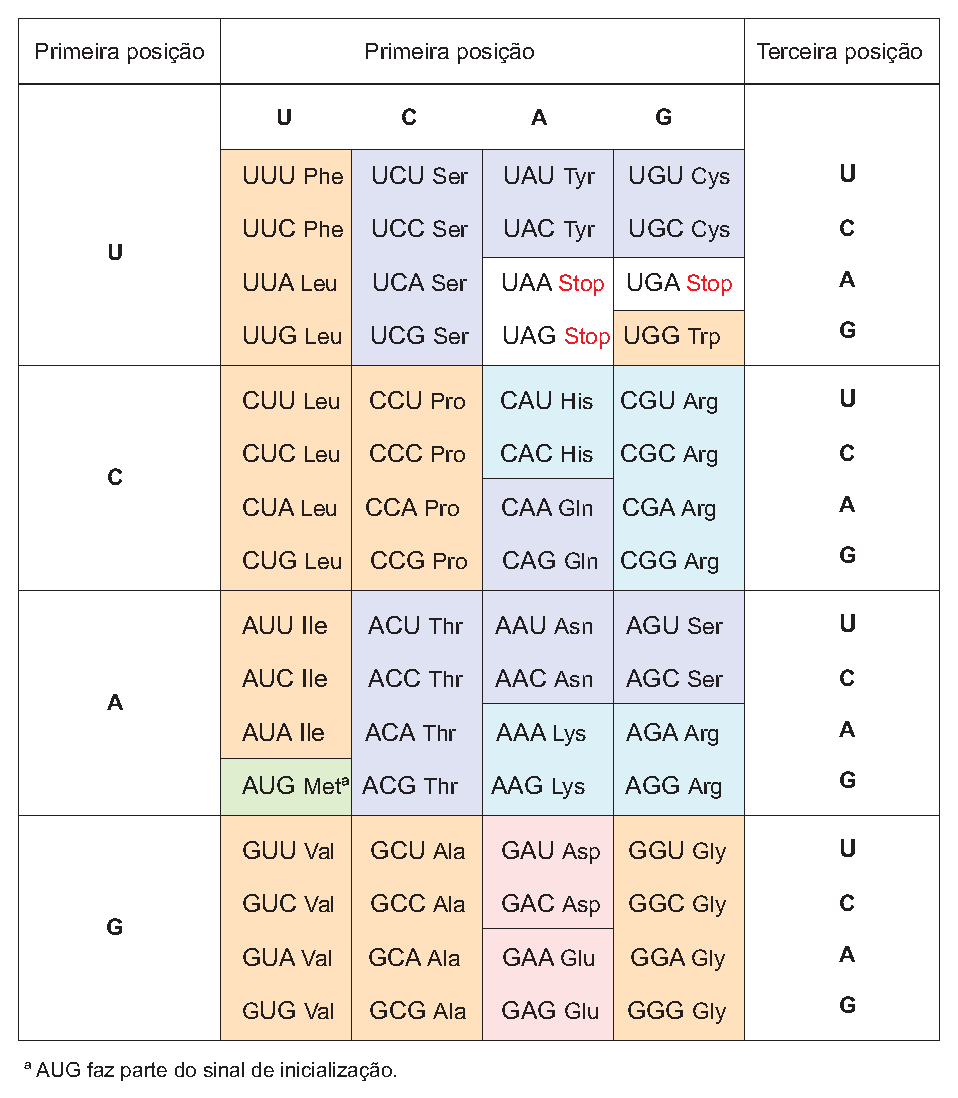
\includegraphics[angle=0,width=0.8\textwidth]{imagens//1995voet-aa}
\end{table}

Depois, é feito o pareamento do segundo tRNA, os aminoácidos são ligados e o primeiro tRNA é liberado. Esse processo é repetido até que apareça um sinal de terminação no mRNA, que vai resultar na formação de uma cadeia polipeptídica.

As proteínas são compostos orgânicos constituídos por aminoácidos unidos através de ligações peptídicas. Elas estão envolvidas em todos os processos biológicos dos seres vivos, como nas funções estruturais catalizadoras e reguladoras~\citep{liu:2006}.


\subsection{\textit{Pipelines} em projetos genoma} \label{sec:pipeline}

Em projetos de genomas, o sistema computacional é chamado \textit{pipeline}~\citep{Lemos:2004}, e é desenvolvido no laboratório de bioinformática. Descrevemos nesta seção, os \textit{pipelines} da antiga tecnologia Sanger e as modernas, chamadas de sequenciamento de nova geração.

    Já nas atuais tecnologias de processamento de alto desempenho, o \textit{pipeline} é dividido em outras fases, e fases semelhantes com objetivos diferentes.  A primeira fase o "mapeamento", busca alinhar os Expressed Sequence Tags (ESTs) obtidos durante um transcritoma com os de um genoma de referência, às vezes, o genoma do próprio organismo de onde os ESTs derivaram. No entanto, outros organismos podem ser utilizados. A fase de anotação apresenta certas diferenças tendo como principal objetivo  a identificação de RNAs não codificadores (ncRNA).


\subsubsection{Técnica: \textit{Sanger}}

Na antiga tecnologia de sequenciamento Sanger, o \textit{pipeline} é, em geral, dividido em três fases, \textbf{submissão}, \textbf{montagem} e \textbf{anotação}. A submissão visa receber as sequências geradas por sequenciadores automáticos a partir de experimentos realizados nos laboratórios de Biologia Molecular, transformando-as em cadeias de caracteres e armazenando-as em bancos de dados. Nota-se que estas sequências são fragmentos de DNA ou de RNA, pois a tecnologia sanger não consegue sequenciar o DNA inteiro nem mesmo mesmo uma molécula inteira de RNA.


\begin{figure} [htb!]
\centering
\fbox{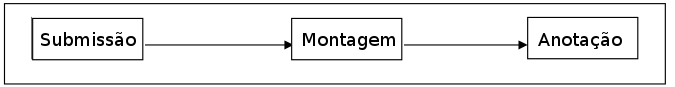
\includegraphics[angle=0,width=0.8\textwidth]{imagens//pipelineSange.png}}
\caption{\textit{pipeline} Sanger. \label{fig:pipeline-Sange}}
\end{figure}

Durante a fase de montagem, as sequências que provavelmente vieram da mesma região do DNA devem ser agrupadas. Cada grupo constituído de duas ou mais sequências é denominado de \textit{contig}, tendo cada \textit{contig} uma sequência resultante (consenso) do agrupamento de todas as sequências que o formam. As sequências que não puderam ser agrupadas são denominadas de \textit{singlets}. 

A última fase, denominada de anotação, consiste em associar funções biológicas às sequências resultantes da fase de montagem (consensos das \textit{contig} e \textit{singlets}), tomando funções conhecidas de sequências similares que estão disponibilizadas em bancos de dados biológicos públicos. Essa fase é dividida em duas etapas: automática e manual.

A anotação automática compara as sequências geradas no projeto com sequências de bancos de dados privados e/ou públicos~\citep{benson2006genbank:2006}. A comparação de duas sequências visa encontrar quais partes das sequências são parecidas ou similares. Dizemos que duas sequências são similares quando são "aproximadamente iguais", ou seja, têm exatamente os mesmos caracteres, com poucos caracteres diferentes, neste caso, podemos inferir que as duas sequências exercem o mesmo "papel biológico" ou têm a mesma função. Existem alguns métodos de comparação aproximada de sequências como BLAST~\citep{altschul1990basic:1990} e FASTA~\citep{pearson1988improved:1988}, bastante utilizados para inferir funções para as sequências identificadas em um projeto genoma.

Na anotação manual, são utilizadas as informações da anotação automática, bem como o conhecimento do biólogo, para determinar a função que vai ser associada efetivamente à sequência analisada.

Na \textbf{submissão} de um projeto genoma feito em sequenciadores Sanger, depois da recepção dos arquivos com os resultados do sequenciamento de cada fragmento (também denominado \textit{read}), um programa chamado \textit{Phred}~\citep{ewing1998base:1998}, traduzir as informações recebidas em sequências de letras contendo as bases identificadas e as probabilidades de erros associadas a cada base, gerando dois arquivos com extensão (\textit{.phd}), para cada \textit{read}. Depois, o programa \textit{Phd2Fasta} cria, pelo \textit{Phred}, dois arquivos texto no formato FASTA: um contendo a sequência de bases nitrogenadas e outro contendo os valores das probabilidades de erro.

A fase de submissao contém um grande numero de sequências, porém, nem todas são utilizadas nos próximos passos. Para ser utilizada, uma sequência deve possuir uma probabilidade de erro suficientemente baixa, sendo essa probabilidade determinada de acordo com cada projeto. Serão aceitas as sequências com qualidade mínima, o que aumenta a confiabilidade nos dados. 


O sequenciamento Sanger envolve cópias do DNA do organismo estudado, inseridas em um outro organismo. Assim, as sequências podem não pertencer ao organismo que está sendo estudado. Um programa chamado \textit{Cross match} visa identificar e retirar vetores e contaminantes das sequências. 
  

Na fase de \textbf{montagem}, são usado em geral dois programas, o \textit{CAP3}~\citep{huang1999cap3:1999} ou o \textit{Phrap}~\citep{green1994phrap:1994}. Estes programas geram arquivos FASTA contendo: as sequências de todos os \textit{singlets}; dados sobre a composição e sequências dos \textit{contigs}; e informações gerais sobre a montagem dos fragmentos de DNA.

Existe dois tipos de projetos de sequenciamento: genômico e transcritômico. No primeiro caso, para a identificação dos possíveis genes presentes nos \textit{contigs} e \textit{singlets} obtidos durante a montagem, utiliza-se o programa \textit{Glimmer}~\citep{salzberg1998microbial:1998}, para identificar ORFs. No caso de transcritomas, os \textit{contigs} e \textit{singlets} já codificam um gene, e assim, não há necessidade de se utilizar o \textit{Glimmer} para fazer a idenficação.


Por fim, na fase de \textbf{anotação} é utilizado o programa BLAST para fazer a comparação das sequências identificadas com bancos de dados de sequências cujas funções já são conhecidas na fase de anotação automática. Depois de feito esse procedimento, os bíologos podem proceder a anotação manual das sequências de acordo com seus conhecimentos.


Em todas etapas anteriormente descritas, são armazenadas estatísticas sobre o projeto, sendo algumas delas: o número de sequências aceitas e rejeitadas na fase de submissão, número de \textit{contigs} e \textit{singlets} encontrados (montagem), além de anotações manuais e automáticas.  


\subsubsection{Técnica: Alto-Desempenho} \label{sec:Sequenciamento}


No início da década de 2000, novas técnicas de sequenciamento massivamente pararelas revolucionaram a forma de realizar o sequenciamento do DNA. Com um custo muito baixo em comparação com o método Sanger, permitindo o sequenciamento de milhões de sequências, esses métodos tiveram um grande impacto nas áreas de pesquisa onde se realiza sequenciamento do DNA, e assim abriram novas frentes de pesquisas, como o estudo de DNAs antigos em mamutes, e diversidade ecológica por meio do sequenciamento de DNA de amostras ambientais~\citep{mardis2008next:2008}.

Nesta seção estudaremos o funcionamento de dois sequenciadores, o 454-FLX da Roche e o Illumina

\subsubsection*{454-FLX Roche} \label{sec:454}

O 454-FLX foi o primeiro sequenciador a aparecer no mercado, em 2004, utilizando uma técnica de sequenciamento conhecida com o nome de pirosequenciamento\citep{ronaghi1998sequencing:1998}. Essa técnica busca incorporar os nucleotídeo a uma fita de DNA por meio da enzima DNA polimerase que acarreta a liberação de pirofostato. Com isso a molécula inicia uma série de reações químicas cujo produto final é a liberação de luz. A detecção da luz e obtida por um sensor que permite a determinação das bases de uma sequência de DNA.


O 454-FLX Roche gera sequências de cerca de 250 a 600 bases de comprimento. Depois desse processamento, sequências com baixa qualidade são removidas, obtendo em cerca de milhões de bases com boa qualidade em média, com cerca de 1 milhão de \textit{reads}. O tamanho das sequências obtidas com o sequenciamento 454-FLX é menor que o sequenciamento Sanger, mas foi utilizado com sucesso no sequenciamento de genomas virais de bactériais com uma qualidade bastante alta.

Em geral, \textit{pipelines} para o 454 Roche envolvem uma fase de \textbf{filtragem}, que retira sequências com qualidades ruins, uma fase de \textbf{montagem}, feita por sobreposição de extremidades similares de sequências de entrada, e uma fase de \textbf{análise}, que inclui anotação.

\begin{figure} [htb!]
\centering
\fbox{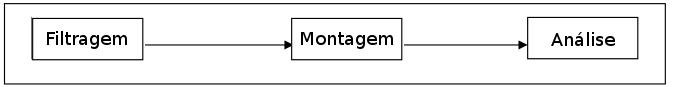
\includegraphics[angle=0,width=0.8\textwidth]{imagens//pipeline454.png}}
\caption{Um \textit{pipeline} genérico para o sequenciamento do 454 Roche. \label{fig:pipeline-454-FLX}}
\end{figure}


\subsubsection*{Illumina} \label{sec:Illumina}

A técnica de sequenciamento utilizada no Illumina incorpora um nucleotídeo por vez à sequência que está sendo determinada. Primeiro, realiza-se a amplificação de fragmentos do DNA, sendo incorporadoes adaptadores no início e fim de cada um dos fragmentos de DNA, que são anexandos a uma superfície. Depois disso, a DNA polimerase é utilizada para a produção de grupos de sequências, cada grupo contendo aproximadamente 1 milhão de cópias de fragmentos de DNA original.

Depois de amplificado o DNA, realiza-se o processo de sequenciamento em si. Nesse estágio, nucleotídeos fosforecentes são adicionados às moléculas de DNA amplificadas. Com a incorporação concluída, processa-se a imagem com as luzes oriundas dos nucleotídeos fosforecentes. Esse processo continua por um determinado número de ciclos, sendo controlado pelo operador do sequenciador, e podem ser construídas as sequências com 25 a 90 bases de comprimento, o que gera bilhões de bases sequenciadas, e cerca de 10 milhões de \textit{reads}~\citep{dohm2008substantial:2008}.

Um \textit{pipeline} para Illumina inclui uma fase de \textbf{mapeamento}, onde as \textit{reads} de tamanho curto são mapeadas em um genoma de referência, e uma fase de \textbf{análise}, que inclui estatísticas de cobertura de \textbf{análise} de expressão diferencial, por exemplo. 

\begin{figure} [htb!]
\centering
\fbox{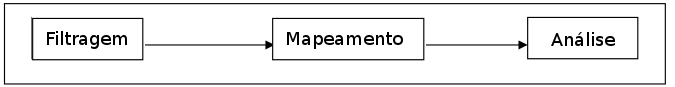
\includegraphics[angle=0,width=0.8\textwidth]{imagens//pipelineIllumina.png}}
\caption{Um \textit{pipeline} genérico para o sequenciamento do Illumina. \label{fig:pipeline-Illumina}}
\end{figure}

